

\begin{frame}{\ft{Document Viewers Augmented With APIs}}

\doubleFrame{Another strategy for realizing interactive publications is 
to link documents with publisher's APIs, or APIs maintained 
by other cultural or educational institutions.}

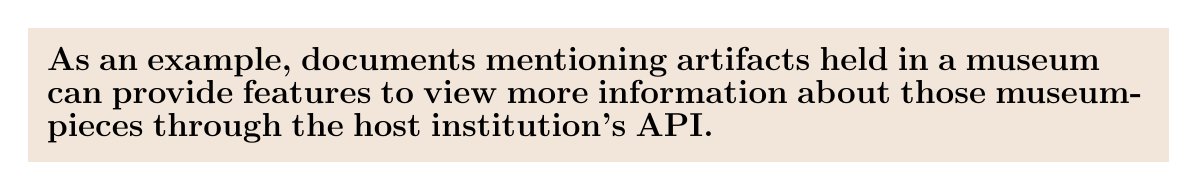
\begin{tikzpicture}
\nodeincludegraphicsTR{2.7cm}{2cm}{pics/Pub-3.png}

 \node [anchor=west,fill=brown!20!white,inner sep=7, text width=14cm]
  (longnote) at (2.5,10) {%  %{\color{rb!85!red}{
  {\cframedbox{\large \textbf{As an example, documents 
mentioning artifacts held in a museum can provide features to 
view more information about those museum-pieces through the host 
institution's API. 
}}}};

\end{tikzpicture}


\end{frame}

